\documentclass{standalone}
\usepackage{tikz}
\usetikzlibrary{patterns, positioning}
\usepackage[sfdefault]{ClearSans} %% option 'sfdefault' activates Clear Sans as the default text font
\usepackage[T1]{fontenc}

\begin{document}
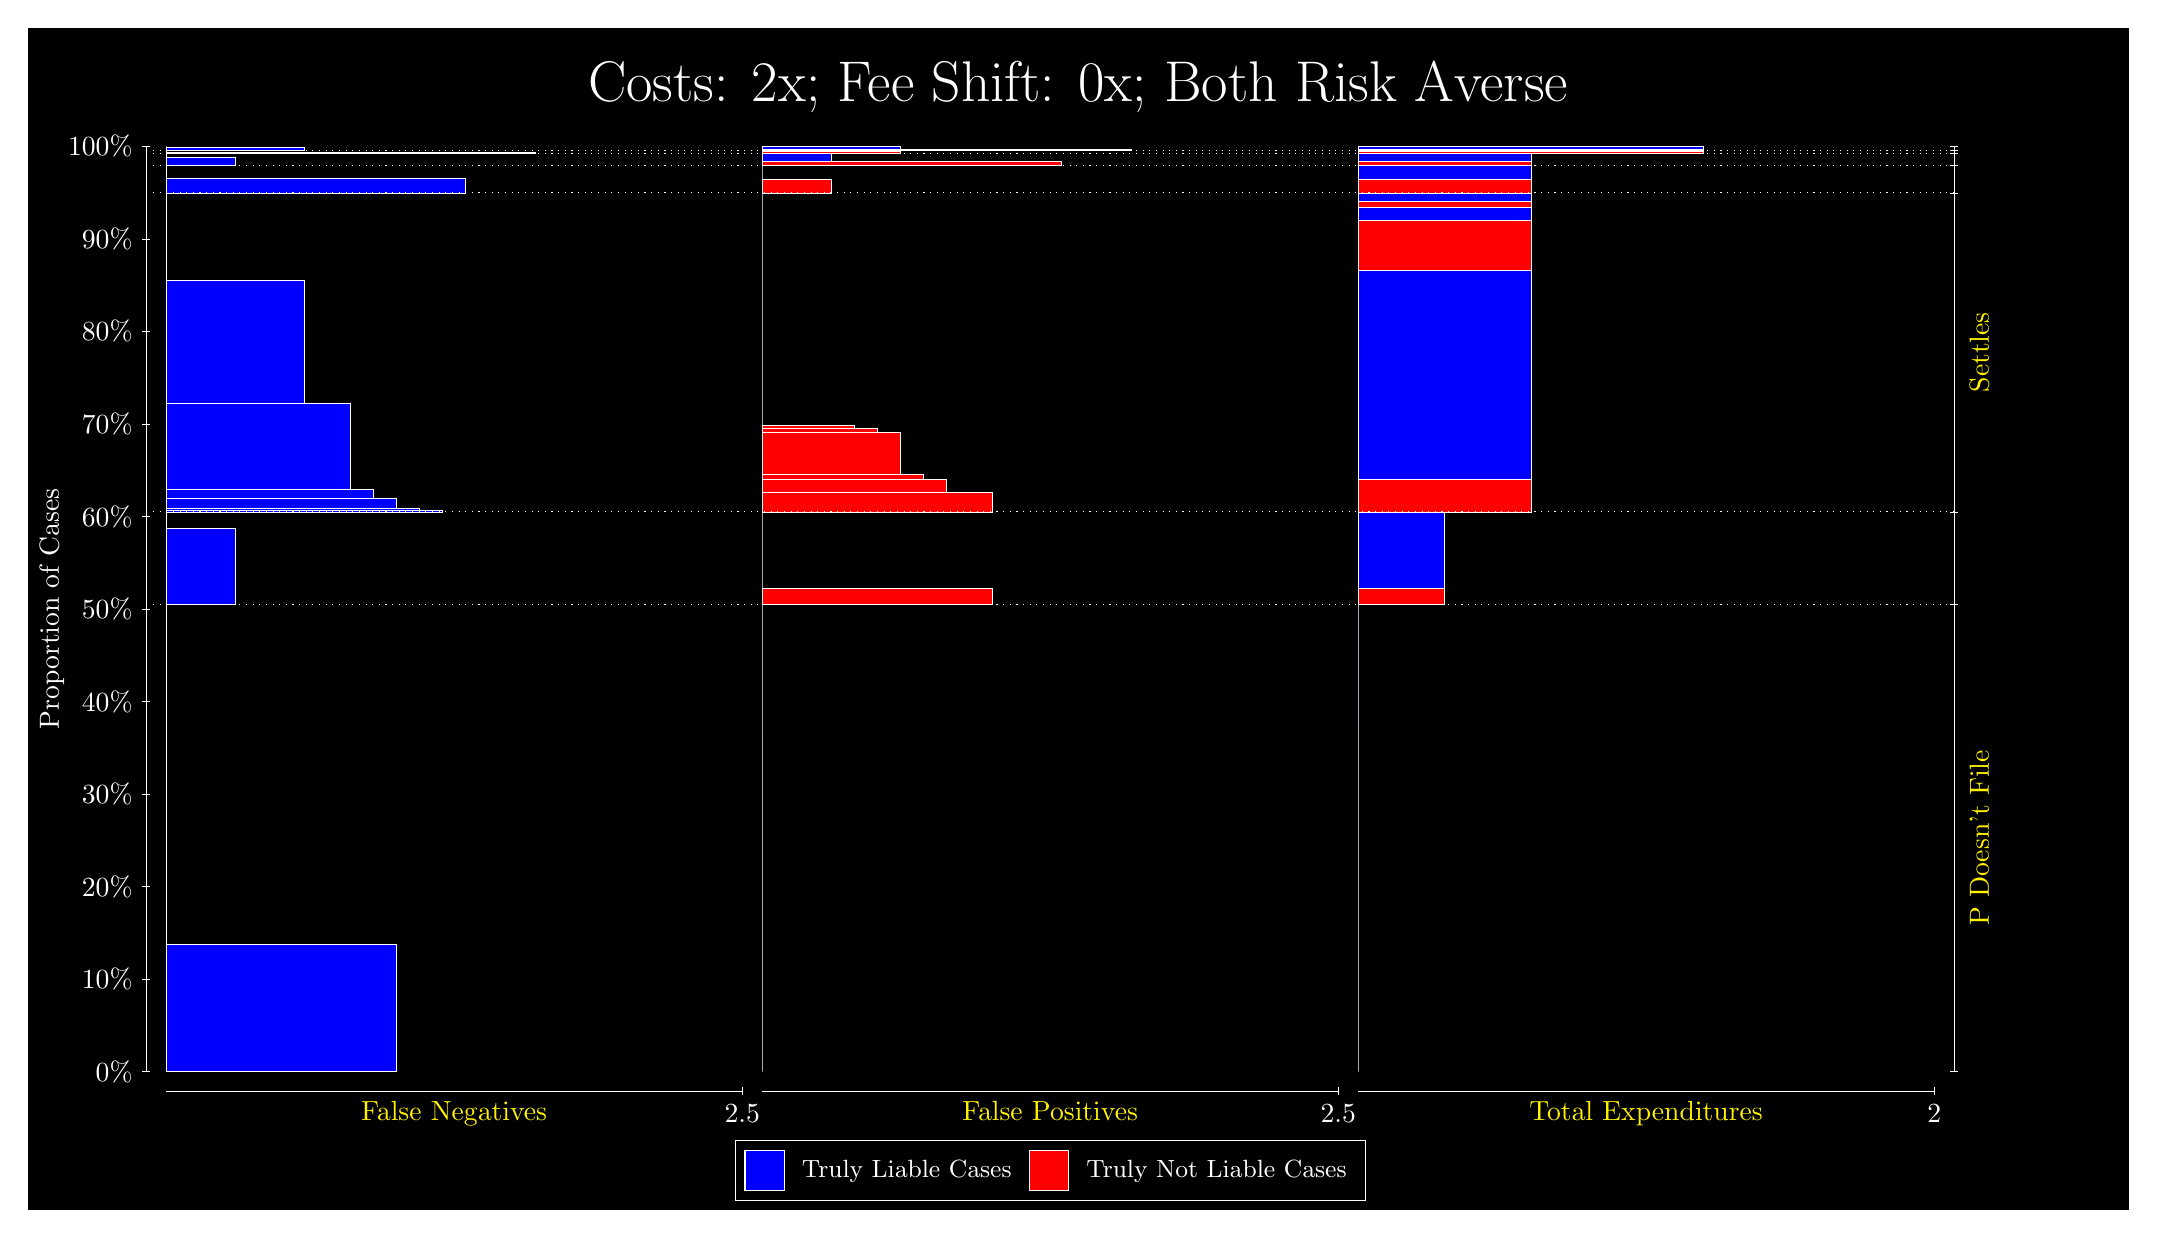
\begin{tikzpicture}
\draw[fill=black] (0,0) rectangle (26.667,15);
\draw[text=white] (0,13.5) rectangle (26.667,15) node[midway] {\huge Costs: 2x; Fee Shift: 0x; Both Risk Averse};
\draw[white, very thin] (1.5,1.75) -- (1.5,13.5);
\node[rotate=90, text=white, anchor=center] at (0.3, 7.625) {Proportion of Cases};
\draw[white, very thin] (1.45,1.75) -- (1.55,1.75);
\node[text=white, anchor=east] at (1.45, 1.75) {0\%};
\draw[white, very thin] (1.45,2.925) -- (1.55,2.925);
\node[text=white, anchor=east] at (1.45, 2.925) {10\%};
\draw[white, very thin] (1.45,4.1) -- (1.55,4.1);
\node[text=white, anchor=east] at (1.45, 4.1) {20\%};
\draw[white, very thin] (1.45,5.275) -- (1.55,5.275);
\node[text=white, anchor=east] at (1.45, 5.275) {30\%};
\draw[white, very thin] (1.45,6.45) -- (1.55,6.45);
\node[text=white, anchor=east] at (1.45, 6.45) {40\%};
\draw[white, very thin] (1.45,7.625) -- (1.55,7.625);
\node[text=white, anchor=east] at (1.45, 7.625) {50\%};
\draw[white, very thin] (1.45,8.8) -- (1.55,8.8);
\node[text=white, anchor=east] at (1.45, 8.8) {60\%};
\draw[white, very thin] (1.45,9.975) -- (1.55,9.975);
\node[text=white, anchor=east] at (1.45, 9.975) {70\%};
\draw[white, very thin] (1.45,11.15) -- (1.55,11.15);
\node[text=white, anchor=east] at (1.45, 11.15) {80\%};
\draw[white, very thin] (1.45,12.325) -- (1.55,12.325);
\node[text=white, anchor=east] at (1.45, 12.325) {90\%};
\draw[white, very thin] (1.45,13.5) -- (1.55,13.5);
\node[text=white, anchor=east] at (1.45, 13.5) {100\%};

\draw[white, very thin] (24.457,1.75) -- (24.457,13.5);
\draw[white, very thin] (24.407,1.75) -- (24.507,1.75);
\node[anchor=west] at (24.407, 1.75) {};
\draw[white, very thin] (24.407,7.6837) -- (24.507,7.6837);
\node[anchor=west] at (24.407, 7.6837) {};
\draw[white, very thin] (24.407,8.8587) -- (24.507,8.8587);
\node[anchor=west] at (24.407, 8.8587) {};
\draw[white, very thin] (24.407,12.909) -- (24.507,12.909);
\node[anchor=west] at (24.407, 12.909) {};
\draw[white, very thin] (24.407,13.255) -- (24.507,13.255);
\node[anchor=west] at (24.407, 13.255) {};
\draw[white, very thin] (24.407,13.413) -- (24.507,13.413);
\node[anchor=west] at (24.407, 13.413) {};
\draw[white, very thin] (24.407,13.444) -- (24.507,13.444);
\node[anchor=west] at (24.407, 13.444) {};
\draw[white, very thin] (24.407,13.5) -- (24.507,13.5);
\node[anchor=west] at (24.407, 13.5) {};

\draw[white, very thin, fill=blue] (1.75,1.75) rectangle (4.6775,3.366);
\draw[white, very thin, fill=red] (1.75,3.366) rectangle (1.75,7.6837);
\draw[white, very thin, fill=blue] (1.75,7.6837) rectangle (2.6283,8.6554);
\draw[white, very thin, fill=red] (1.75,8.6554) rectangle (1.75,8.8587);
\draw[white, very thin, fill=blue] (1.75,8.8587) rectangle (5.2631,8.8736);
\draw[white, very thin, fill=blue] (1.75,8.8736) rectangle (4.9703,8.9041);
\draw[white, very thin, fill=blue] (1.75,8.9041) rectangle (4.6775,9.034);
\draw[white, very thin, fill=blue] (1.75,9.034) rectangle (4.3848,9.1428);
\draw[white, very thin, fill=blue] (1.75,9.1428) rectangle (4.092,10.235);
\draw[white, very thin, fill=blue] (1.75,10.235) rectangle (3.5065,11.805);
\draw[white, very thin, fill=red] (1.75,11.805) rectangle (1.75,12.909);
\draw[white, very thin, fill=blue] (1.75,12.909) rectangle (5.5558,13.088);
\draw[white, very thin, fill=red] (1.75,13.088) rectangle (1.75,13.255);
\draw[white, very thin, fill=blue] (1.75,13.255) rectangle (2.6283,13.362);
\draw[white, very thin, fill=red] (1.75,13.362) rectangle (1.75,13.413);
\draw[white, very thin, fill=blue] (1.75,13.413) rectangle (6.4341,13.426);
\draw[white, very thin, fill=red] (1.75,13.426) rectangle (1.75,13.444);
\draw[white, very thin, fill=blue] (1.75,13.444) rectangle (3.5065,13.487);
\draw[white, very thin, fill=red] (1.75,13.487) rectangle (1.75,13.5);
\draw[white, very thin, fill=red] (9.3189,1.75) rectangle (9.3189,6.0677);
\draw[white, very thin, fill=blue] (9.3189,6.0677) rectangle (9.3189,7.6837);
\draw[white, very thin, fill=red] (9.3189,7.6837) rectangle (12.246,7.887);
\draw[white, very thin, fill=blue] (9.3189,7.887) rectangle (9.3189,8.8587);
\draw[white, very thin, fill=red] (9.3189,8.8587) rectangle (12.246,9.1026);
\draw[white, very thin, fill=red] (9.3189,9.1026) rectangle (11.661,9.2697);
\draw[white, very thin, fill=red] (9.3189,9.2697) rectangle (11.368,9.3378);
\draw[white, very thin, fill=red] (9.3189,9.3378) rectangle (11.075,9.8679);
\draw[white, very thin, fill=red] (9.3189,9.8679) rectangle (10.783,9.9231);
\draw[white, very thin, fill=red] (9.3189,9.9231) rectangle (10.49,9.9628);
\draw[white, very thin, fill=blue] (9.3189,9.9628) rectangle (9.3189,12.909);
\draw[white, very thin, fill=red] (9.3189,12.909) rectangle (10.197,13.077);
\draw[white, very thin, fill=blue] (9.3189,13.077) rectangle (9.3189,13.255);
\draw[white, very thin, fill=red] (9.3189,13.255) rectangle (13.125,13.306);
\draw[white, very thin, fill=blue] (9.3189,13.306) rectangle (10.197,13.413);
\draw[white, very thin, fill=red] (9.3189,13.413) rectangle (11.075,13.431);
\draw[white, very thin, fill=blue] (9.3189,13.431) rectangle (9.3189,13.444);
\draw[white, very thin, fill=red] (9.3189,13.444) rectangle (14.003,13.457);
\draw[white, very thin, fill=blue] (9.3189,13.457) rectangle (11.075,13.5);
\draw[white, very thin, fill=red] (16.888,1.75) rectangle (16.888,6.0677);
\draw[white, very thin, fill=blue] (16.888,6.0677) rectangle (16.888,7.6837);
\draw[white, very thin, fill=red] (16.888,7.6837) rectangle (17.986,7.887);
\draw[white, very thin, fill=blue] (16.888,7.887) rectangle (17.986,8.8587);
\draw[white, very thin, fill=red] (16.888,8.8587) rectangle (19.083,9.2697);
\draw[white, very thin, fill=blue] (16.888,9.2697) rectangle (19.083,11.932);
\draw[white, very thin, fill=red] (16.888,11.932) rectangle (19.083,12.557);
\draw[white, very thin, fill=blue] (16.888,12.557) rectangle (19.083,12.732);
\draw[white, very thin, fill=red] (16.888,12.732) rectangle (19.083,12.8);
\draw[white, very thin, fill=blue] (16.888,12.8) rectangle (19.083,12.909);
\draw[white, very thin, fill=red] (16.888,12.909) rectangle (19.083,13.077);
\draw[white, very thin, fill=blue] (16.888,13.077) rectangle (19.083,13.255);
\draw[white, very thin, fill=red] (16.888,13.255) rectangle (19.083,13.306);
\draw[white, very thin, fill=blue] (16.888,13.306) rectangle (19.083,13.413);
\draw[white, very thin, fill=red] (16.888,13.413) rectangle (21.279,13.431);
\draw[white, very thin, fill=blue] (16.888,13.431) rectangle (21.279,13.444);
\draw[white, very thin, fill=red] (16.888,13.444) rectangle (21.279,13.457);
\draw[white, very thin, fill=blue] (16.888,13.457) rectangle (21.279,13.5);
\draw[white, dotted] (1.5,7.6837) -- (24.457,7.6837);
\draw[white, dotted] (1.5,8.8587) -- (24.457,8.8587);
\draw[white, dotted] (1.5,12.909) -- (24.457,12.909);
\draw[white, dotted] (1.5,13.255) -- (24.457,13.255);
\draw[white, dotted] (1.5,13.413) -- (24.457,13.413);
\draw[white, dotted] (1.5,13.444) -- (24.457,13.444);
\draw[white, very thin] (1.75,1.5) -- (9.0689,1.5);
\node[text=yellow, anchor=north] at (5.4094, 1.5) {False Negatives};
\draw[white, very thin] (9.0689,1.45) -- (9.0689,1.55);
\node[text=white, anchor=north] at (9.0689, 1.45) {2.5};

\draw[white, very thin] (9.3189,1.5) -- (16.638,1.5);
\node[text=yellow, anchor=north] at (12.978, 1.5) {False Positives};
\draw[white, very thin] (16.638,1.45) -- (16.638,1.55);
\node[text=white, anchor=north] at (16.638, 1.45) {2.5};

\draw[white, very thin] (16.888,1.5) -- (24.207,1.5);
\node[text=yellow, anchor=north] at (20.547, 1.5) {Total Expenditures};
\draw[white, very thin] (24.207,1.45) -- (24.207,1.55);
\node[text=white, anchor=north] at (24.207, 1.45) {2};

\node[text=yellow, centered, rotate=90] at (24.777, 4.7168) {P Doesn't File};

\node[text=yellow, centered, rotate=90] at (24.777, 10.884) {Settles};





\draw (12.978300999999998,1.5) node[draw=none] (baseCoordinate) {};
\begin{scope}[align=center]
        \matrix[scale=0.5, draw=white, below=0.5cm of baseCoordinate, nodes={draw}, column sep=0.1cm]{
            \node[rectangle, draw, minimum width=0.5cm, minimum height=0.5cm, fill=blue] {}; &
            \node[draw=none, font=\small, text=white] (B) {Truly Liable Cases}; &
            \node[rectangle, draw, minimum width=0.5cm, minimum height=0.5cm, fill=red] {}; &
            \node[draw=none, font=\small, text=white] (B) {Truly Not Liable Cases}; \\
            };
\end{scope}

\end{tikzpicture}
\end{document}